%
% This work is licensed under a Creative Commons Attribution-ShareAlike 4.0 International License.
%

\documentclass[10pt, a5paper, twoside, openany]{memoir}

\setsecnumdepth{subsection}

\title{Introduction to Quantum Mechanics}
\author{Joseph D. MacMillan}
\date{}


\usepackage{graphicx}
\usepackage{color} 
\usepackage{amsmath, amssymb}
\usepackage{libertinus}
\usepackage{microtype}
\usepackage{layout}
\usepackage[most]{tcolorbox}
\tcbuselibrary{skins,breakable}
\usepackage[hang, small, bf]{caption}
\captionsetup[table]{position=top}
\captionsetup[figure]{position=bottom}
\usepackage[hyphens]{url}
\usepackage[hidelinks]{hyperref}
\hypersetup{pdftitle={Introduction to Quantum Mechanics}}
\hypersetup{pdfauthor={Joseph D. MacMillan}}
\urlstyle{rm}


% Set page margins, etc
\setstocksize{9in}{6in}
\settrimmedsize{\stockheight}{\stockwidth}{*}
\settrims{0pt}{0pt}

\setlxvchars %define lenght 65 char of the used font
\settypeblocksize{*}{1.05\lxvchars}{1.7}
\setbinding{20pt} 
\setlength{\headheight}{30pt}
\setlength{\footskip}{20pt}

\setulmargins{90pt}{*}{*}
\setlrmargins{*}{*}{*}
\setheaderspaces{*}{30pt}{*}

\setmarginnotes{0.01pt}{20pt}{\onelineskip}
\checkandfixthelayout

\setcounter{tocdepth}{3}



\newcommand{\uu}{\symbfup{u}}
\newcommand{\grad}{\symbfup{\nabla}}
\newcommand{\curl}{\symbfup{\nabla} \times}
\newcommand{\dfdx}[2]{\frac{\partial {#1}}{\partial {#2}}}
\newcommand{\ddfdx}[2]{\frac{\partial^2 {#1}}{\partial {#2}^2}}
\newcommand{\vort}{\symbfup{\omega}}
\renewcommand\vec{\symbfup}
\newcommand{\unit}[1]{\hat{\vec{#1}}}
\newcommand{\U}{\mathbb{U}}
\newcommand{\V}{\mathbb{V}}
\newcommand{\LL}{\mathbb{L}^2}
\newcommand{\LLLL}{\mathbb{L}^4}

\newcommand{\ket}[1]{| #1 \rangle}
\newcommand{\bra}[1]{\langle #1 |}
\newcommand{\braket}[2]{\langle #1 | #2 \rangle}


%\DeclareMathAlphabet{\mathbfsf}{\encodingdefault}{\sfdefault}{bx}{sl}
\newcommand{\tens}[1]{\mathbfsfit{#1}}


\newcounter{example}[chapter]
\def\theexample{\thechapter.\arabic{example}}
\newenvironment{example}[1][ ]{\refstepcounter{example}
\begin{tcolorbox}[breakable, sharp corners, boxrule = 0pt, frame empty, opacityframe=0, parbox=false]
\textbf{Example \theexample \ -- #1.}
}
{ 
\end{tcolorbox}
}

\newenvironment{theorem}[1][ ]{
\begin{tcolorbox}[breakable, sharp corners, boxrule = 0pt, frame empty, opacityframe=0, parbox=false]
\textbf{#1.}
}
{ 
\end{tcolorbox}
}

\newcounter{problem}[chapter]
\def\theproblem{\thechapter.\arabic{problem}}
\newenvironment{problem}[1][ ]{\refstepcounter{problem} \noindent \textbf{Problem \theproblem \ -- #1.}}{\vspace{0.1in}}


\begin{document}

\frontmatter

\maketitle

\begin{center}


\includegraphics[width=\linewidth]{Figures/fig_cover_wave}

\vspace{1in}

{\small

This version was compiled on \today.  For the most up-to-date version and supplementary material, see \href{https://josephmacmillan.github.io/IntroductionToQuantumMechanics/index.html}{josephmacmillan.github.io/IntroductionToQuantumMechanics}.

\vspace{2in}

This work is licensed under a \href{https://creativecommons.org/licenses/by-sa/4.0/}{Creative Commons Attribution-ShareAlike 4.0 International License}.
}
\end{center}


\newpage

\tableofcontents

\chapter{Preface}

To come. 

\section{Why Open Education?}

This book and the supplementary material are released under a Creative Commons Attribution-ShareAlike 4.0 International License, which means you can do anything you want with this book:  cut out stuff you don't need, use it to build an even better book, download it for free off the web, print it out yourself, give it to your friends (they want a copy, trust me), and anything else you can think of.  The only stipulation is that you give credit where it's due, and release the derivative work under the same license.

Why did I choose this?  Because I've taught university courses and have seen the issues with expensive textbooks: students not being able to afford them, students finding illegal PDF copies online and sharing them, the publishing companies fighting back with various schemes like renting digital copes, and so on.  Especially in advanced physics, little textbooks can be so expensive, and yet I think textbooks are an important and necessary resource, and I want my students to all have a copy.

\section{Thanks}

To come.

\vspace{1in}

Find a typo, mistake, or horrible misconception in this book?  Let me know by creating a new issue at the GitHub page:  

\href{https://github.com/josephmacmillan/IntroductionToQuatumMechanics/issues}{github.com/josephmacmillan/IntroductionToQuantumMechanics/issues}.



\mainmatter

\chapter{The Stern-Gerlach Experiment}

\section{Spin Angular Momentum}

Let's start with a system that is pretty much as far away from the quantum world as possible -- the Earth and Sun, as shown in Figure \ref{fig_sun_earth}.  With its total motion, the Earth has two kinds of angular momentum:  \emph{orbital} angular momentum $\vec{L}$ from its orbit around the sun, and \emph{spin} angular momentum $\vec{S}$, resulting from its 24 hour rotation.  Of course, the spin angular momentum in this case is due to adding up the orbital angular momentum $\vec{L}_i = \vec{r}_i \times \vec{p}_i$ of each of the tiny pieces of the Earth, but we'll keep the distinction because this is definitively not the case in quantum systems as we'll see.  Note that the two kinds of angular momentum for the Earth point in different directions since the rotation axis of the Earth is tilted 23$^\circ$ from the orbital plane.

\begin{figure}
\centering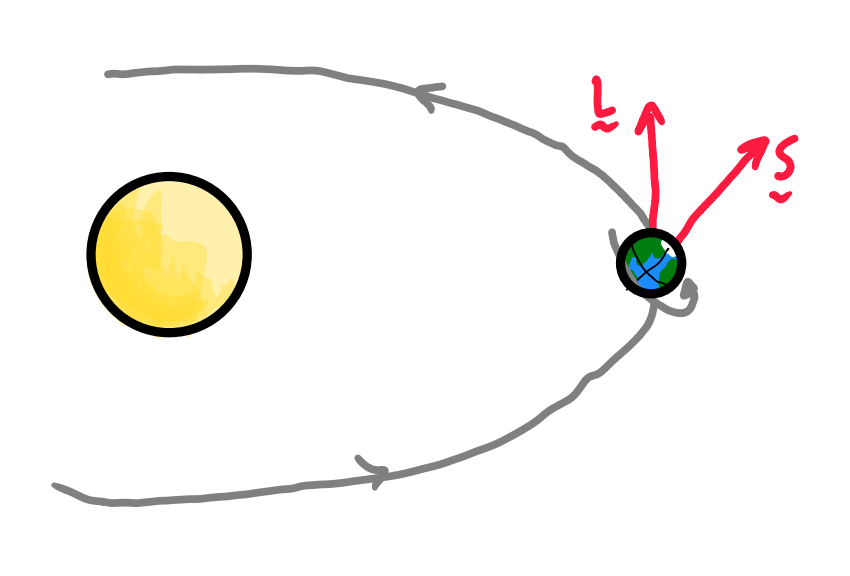
\includegraphics[width=0.5\linewidth]{Figures/Chapter 1/fig_sun_earth.png}
\caption{The Earth goes around the Sun every 365 days (orbital angular momentum) and rotates around its axis every 24 hours (spin angular momentum).}
\label{fig_sun_earth}
\end{figure}

As a simple quantum system, consider an electron in orbit around a proton -- a hydrogen atom.  The electron has orbital angular momentum just like the Earth (depending on what state it's in), and it also has spin angular momentum.  Careful, though, as the electron doesn't rotate like the Earth -- how can it when it has essentially no size or diameter to spin?  Despite this, it has measurable intrinsic angular momentum, which we'll call \emph{spin} $\vec{S}$.  Since spin is a vector, it has components $(S_x, S_y, S_z)$, and thus to specific the spin of the electron we use three different numbers; keep this in mind for later.

Suppose we put a stationary electron in a magnetic field $\vec{B}$.  Since the electron is stationary, the Lorentz force
\[
\vec{F} = q\vec{v} \times \vec{B}
\]
is zero.  But the electron's spin angular momentum gives it a magnetic dipole moment $\vec{\mu}$, and it's then possible for an \emph{inhomogeneous} magnetic field to exert a force (see Griffiths \emph{Introduction to Electrodynamics}, fourth edition, section 6.2)
\begin{equation}
\vec{F} = \grad (\vec{\mu} \cdot \vec{B}).
\end{equation}



%
%
%

\section{The Stern-Gerlach Experiment}

The 

%
%
%

\section{Extending the Experiments}

The 

%
%
%



\section*{Problems}
\addcontentsline{toc}{section}{Problems}
\markright{Problems}%

\begin{problem}[Electron spin]
How fast would the surface of an electron be going if it had ....
\end{problem}


\chapter{Examples of Discrete Systems}

\section{An Electron in a Magnetic Field}

To come.
%
%
%

\section{Neutrino Oscillations}

Neutrinos -- little neutral particles created in huge numbers during nuclear reactions -- were long though to be massless.  But during the 1980s and 1990s the \emph{solar neutrino problem} became undeniable: neutrino detection experiments on Earth were missing about half of the expected number of neutrinos made in the core of the sun during hydrogen burning.  There were only two possibilities:  either our model of the sun was way off\footnote{One of my undergraduate professors was a solar physicists, and according to him there was no way the solar models could be that wrong, so really there's only one possible explanation -- something was wrong with our understanding of neutrinos.} or something happened to the neutrinos on their way to us.

The correct explanation turned out to be something called \emph{neutrino oscillations}, and the theory earned the Nobel prize.  In short, \emph{electron} neutrinos are created in the core of the sun, but on their way to Earth some of them turn into \emph{muon} neutrinos -- don't worry too much about the names or why there's more than one kind of neutrino; the main idea is that neutrinos can oscillate back and forth between these two different types (actually, there's a \emph{third} type, a tau neutrino, but we'll ignore that for simplicity).

As a slightly simplified model for neutrino mixing, we'll suppose the state of any neutrino -- I'll call this the ``flavour state,'' since particle physicists call the type of particle its flavour for some reason -- can be written as a superposition of an electron neutrino state and a muon neutrino state:
\begin{equation}
\ket{\nu} = a \ket{e} + b \ket{\mu}.
\end{equation}
This is a two-state system, something we've already studied in detail, so the physics of neutrinos is pretty much the same as spin-1/2 systems or photon polarizations.  To see how neutrinos oscillate, though, we'll have to calculate how this state evolves in time, meaning we'll need the Hamiltonian of the system.

The Hamiltonian, of course, is just the total energy, so we'll start with the relativistic energy of any particle (unfortunately, neutrinos are inherently relativistic objects -- it's hard to slow them down), 
\[
E = \sqrt{p^2c^2 + m^2 c^4}.
\]
Although neutrinos were originally thought to be massless, it turns out we'll need to give them a very small mass in order for them to oscillate.  That said, it will be a \emph{very} small mass, so it's reasonable to think that their rest energy ($mc^2)$ will be much smaller than their momentum (the $pc$ term), in which case we can write 
\[
E = pc \left( 1 + \frac{m^2c^4}{p^2c^2} \right)^{1/2} \approx pc \left( 1 + \frac{m^2c^4}{2p^2c^2} \right),
\]
or
\begin{equation}
\label{eq_relE}
E = pc + \frac{m^2c^3}{2p}.
\end{equation}
For reasons we won't see until we solve the whole problem, I'm going to write the Hamiltonian as
\begin{equation}
\hat{H} \to \begin{pmatrix}
pc + (m_1^2 + m_2^2) c^3/4p & (m_1^2 - m_2^2)c^3/4p \\
(m_1^2 - m_2^2)c^3/4p &pc + (m_1^2 + m_2^2) c^3/4p 
\end{pmatrix}
\end{equation}
where $m_1$ and $m_2$ are two different masses.  You might think that $m_1$ is the mass of the electron neutrino and $m_2$ is that of the muon neutrino, but that's not quite the case; hold tight and we'll see what that means.

Before we find the energy eigenvalues and eigenstates, consider for a moment what the Hamiltonian would look like if the neutrinos were in fact \emph{massless}; then
\[
\hat{H} \to \begin{pmatrix}
pc & 0 \\
0 & pc 
\end{pmatrix}.
\]
This matrix is diagonal, so the possible energies are easy to read off: they're both the same, $E = pc$ as we'd expect for a massless relativistic particle.  The eigenstates of the matrix are just the flavour basis states, $\ket{e}$ and $\ket{\mu}$, so the implication is that both neutrinos have the same energy.  More importantly, though, the flavour states -- which are also the energy eigenstates -- are stationary states, so neutrino oscillations simply wouldn't happen.  Once an electron neutrino is created during a reaction, it will stay an electron neutrino forever.  Actually, it's possible to have massive neutrinos and still have the flavour states be stationary, as long as the masses are the same.  In this case the matrix remains diagonal and we reach the same conclusions; evidently it's the \emph{different} masses of the two neutrinos that lead to oscillations.

Okay, let's find the energies of the full Hamiltonian.  For ease of writing stuff out, I'm going to write the Hamiltonian as
\[
\hat{H} \to \begin{pmatrix}
h & g \\
g & h 
\end{pmatrix},
\]
where $h = pc + (m_1^2 + m_2^2) c^3/4p$ and $g = (m_1^2 - m_2^2)c^3/4p$.  The characteristic equation is
\[
\begin{vmatrix}
h - E & g \\
g & h - E
\end{vmatrix} = 0,
\]
which has solutions
\begin{equation}
E_1 = h + g = pc + (m_1^2 + m_2^2) c^3/4p + (m_1^2 - m_2^2)c^3/4p = pc + m_1^2 c^3 / 2p
\end{equation}
and
\begin{equation}
E_2 = h - g = pc + (m_1^2 + m_2^2) c^3/4p - (m_1^2 - m_2^2)c^3/4p = pc + m_2^2 c^3 / 2p.
\end{equation}
Now you can see why I chose the exact Hamiltonian I did -- we get exactly the energies we expect based on equation \ref{eq_relE}.  As long as the masses are different, these are two distinct energies.

Now that we have the energy eigenvalues, we can get the corresponding states as well.  For $E = E_1 = h + g$, the eigenvalue equation is
\[
\hat{H} \ket{E_1} = E_1 \ket{E_1},
\]
or, in matrix notation,
\[
\begin{pmatrix}
h & g \\
g & h
\end{pmatrix} \begin{pmatrix}  \alpha \\ \beta \end{pmatrix} = (h+g) \begin{pmatrix}  \alpha \\ \beta \end{pmatrix}.
\]
Solving gives $\beta = \alpha$, and after normalizing to find $\alpha = 1/\sqrt{2}$, the eigenstate is 
\begin{equation}
\label{eq_E1}
\ket{E_1} = \frac{1}{\sqrt{2}} \ket{e} + \frac{1}{\sqrt{2}} \ket{\mu}.
\end{equation}
Similarly, the eigenstate associated with energy $E_2 = h - g$ is
\begin{equation}
\label{eq_E2}
\ket{E_2} = \frac{1}{\sqrt{2}} \ket{e} - \frac{1}{\sqrt{2}} \ket{\mu}.
\end{equation}


This is where things get interesting and a little weird.   According to particle physics, a neutrino is created either as an electron neutrino (state $\ket{e}$) or as a muon neutrino (state $\ket{\mu}$).  But the energy states are a superposition of these flavour states -- evidently the electron neutrino, say, just doesn't \emph{have} a definite energy.  Put another way -- because the energies depend on the two different masses -- we can say the an electron neutrino does not have a definite mass; the $m_1$ isn't an $m_{\nu_e}$.  Alternatively, if we manage to measure the energy (or mass) of an electron neutrino, it's no longer an electron neutrino -- its state collapses to one of the superpositions above and it doesn't have a definite flavour.

We can see how this leads to neutrino oscillations and solves the solar neutrino problem by supposing that, at the centre of the sun, an electron neutrino is created.  The initial state is then
\begin{equation}
\ket{\nu(0)} = \ket{e}.
\end{equation}
I think it's fair to call this neutrino an electron neutrino at this point.

To find the state at a later time, we need to first switch to the energy basis.  For fun, I'll do that by multiplying the state by the identity operator:
\[
\ket{\nu(0)} = \hat{1} \ket{e} = \left( \ket{E_1}\bra{E_1} + \ket{E_2} \bra{E_2} \right) \ket{e}.
\]
Notice that I wrote the identity operator in the energy basis -- this is the mechanism that switches basis for us.  Working out the inner products gives
\begin{equation}
\ket{\nu(0)} =  \frac{1}{\sqrt{2}} \ket{E_1} + \frac{1}{\sqrt{2}} \ket{E_2}
\end{equation}
as you might expect; although it's fair to say this is an electron neutrino, we definitely can't say what the energy of the particle is -- it simply doesn't have one.

Now we can tack on the exponential time factors to find the state at a later time in the usual way.  We get
\[
\ket{\nu(t)} = \frac{e^{-iE_1 t / \hbar}}{\sqrt{2}} \ket{E_1} + \frac{e^{-iE_2 t / \hbar}}{\sqrt{2}} \ket{E_2}.
\]
Finally, I'll switch back to the flavour basis, although this time I'll do it using equations (\ref{eq_E1}) and (\ref{eq_E2}) directly rather than using the identity operator:
\[
\ket{\nu(t)} = \frac{e^{-iE_1 t / \hbar}}{\sqrt{2}} \left( \frac{1}{\sqrt{2}} \ket{e} + \frac{1}{\sqrt{2}} \ket{\mu} \right)  + \frac{e^{-iE_2 t / \hbar}}{\sqrt{2}} \left( \frac{1}{\sqrt{2}} \ket{e} - \frac{1}{\sqrt{2}} \ket{\mu} \right).
\]
Using $E_1 = h + g$ and $E_2 = h -g$ and simplifying things, we get
\[
\ket{\nu(t)} = \frac{1}{2} e^{-iht/\hbar} \left[  \left( e^{-igt/\hbar} + e^{igt/\hbar} \right) \ket{e} +  \left( e^{-igt/\hbar} - e^{igt/\hbar} \right) \ket{\mu} \right].
\]
You might recognize cosine and sine in there, so we'll simplify further, but also note that there's an overall phase factor out in front -- we'll drop that since it doesn't mean anything physically.  Finally, the state at time $t$ is
\begin{equation}
\ket{\nu(t)} = \cos (gt/\hbar) \ket{e} - i \sin(gt/\hbar) \ket{\mu}.
\end{equation}
Take a look at what happens at time
\[
\tau = \frac{\pi \hbar}{g} = \frac{\pi p \hbar}{4c^3} \frac{1}{m_1^2 - m_2^2};
\]
at that point the cosine term goes to zero and the sine term becomes one and our state is
\[
\ket{\nu(\tau)} = \ket{\mu}.
\]
The electron neutrino has oscillated into a muon neutrino!

This is the explanation for the solar neutrino problem, although the full theory is a bit more complex since there are actually three different neutrino flavours.  But the main idea is still the same -- the flavour states are not the energy eigenstates, and are therefore not stationary -- they instead oscillate amongst themselves.



%
%
%



\chapter{The Finite Square Well}

\section{Bound States}

What happens if the walls of our ``box'' weren't quite so high?  Let's find out -- suppose we have a particle in a \emph{finite} square well, defined by the potential energy
\begin{equation}
V(x) = \begin{cases}
V_0, \quad x<-a \\
0, \quad -a<x<a \\
V_0, \quad x>a,
\end{cases}
\end{equation}
where $V_0$ is a positive constant -- the depth of the well as shown in Figure \ref{fig_finite_sqr_well_potential}.  Notice one other difference from the infinite version as well: the well has been centered at $x=0$ so the width of the well is actually $2a$; we'll see why in a little bit. 

\begin{figure}
\centering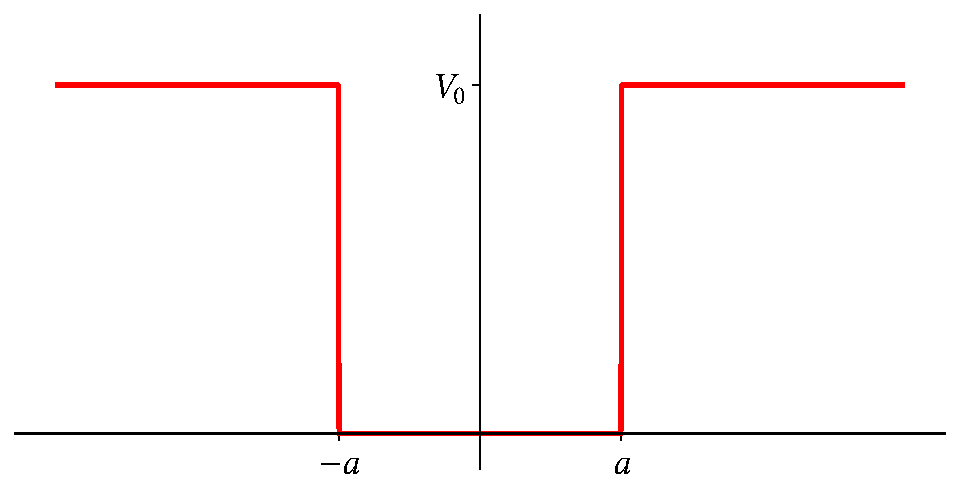
\includegraphics[width=0.7\linewidth]{Figures/Chapter 10/fig_finite_sqr_well_potential.pdf}
\caption{The potential energy of the finite square well.}
\label{fig_finite_sqr_well_potential}
\end{figure}

Actually, probably the biggest difference between the infinite square well and the finite well is what kind of states are allowed.  Classically, for the infinite square well, the particle in the box was always contained and could never escape, regardless of the energy of the particle.  In the finite well, though, if $E>V_0$ the particle would not be trapped in the box and would instead escape to infinity.  As we discussed back in Chapter 8, this case would be an \emph{unbound state}, and unbound states have some additional complications in quantum mechanics -- we'll save those for a later chapter.  In the meantime, we'll only look for bound energy eigenstates, where
\[
E < V_0 \quad \text{(bound states)},
\]
but keep in mind that we'll be missing some of the eigenstates.  One consequence of this is that the energy eigenstates we find here won't be \emph{complete}.

Luckily, finding the bound states is pretty easy.  For $x < -a$, to the left of the well, the energy eigenvalue equation reads
\[
-\frac{\hbar^2}{2m} \frac{d^2 \phi}{dx^2} + V_0 \phi = E\phi,
\]
or, cleaning it up a bit,
\begin{equation}
\frac{d^2\phi}{dx^2} = q^2 \phi,
\end{equation}
where
\begin{equation}
q = \frac{\sqrt{2m(V_0 - E)}}{\hbar}.
\end{equation}
Notice that $q$ is always \emph{real} since we're requiring that $E<V_0$.  This should be a recognizable differential equation; the general solution looks like
\begin{equation}
\phi(x) = A e^{qx} + B e^{-qx} \quad \text{($x<-a$)}.
\end{equation}
Similarly, for $x>a$, the potential energy is again $V = V_0$ so our solution is the same, although we'll have to use different constants:
\begin{equation}
\phi(x) = F e^{qx} + G e^{-qx} \quad \text{($x>a$)}.
\end{equation}

Finally, in the well itself we have $V = 0$, so the solution is the exact same as the infinite square well.  We can write the energy eigenvalue equation as
\begin{equation}
\frac{d^2\phi}{dx^2} = -k^2 \phi,
\end{equation}where
\begin{equation}
k = \frac{\sqrt{2mE}}{\hbar}
\end{equation}
is once again real and positive.  The general solution is 
\begin{equation}
\phi(x) = C \sin(kx) + D\cos(kx) \quad \text{($-a<x<a$)}.
\end{equation}

At the risk of repeating myself unnecessarily, I'll write out the full solution as a piecewise function; it helps to see it all together:
\begin{equation}
\phi(x) = \begin{cases}
A e^{qx} + B e^{-qx}, \quad & x<-a \\
C \sin(kx) + D\cos(kx) , \quad & -a<x<a \\
 F e^{qx} + G e^{-qx}, \quad & x>a.
\end{cases}
\end{equation}
Now all we have to do is find all six constants $A$, $B$, $C$, $D$, $F$, and $G$, plus of course our allowed energy $E$, which is buried inside $q$ and $k$.  To do that we use \emph{boundary conditions} as usual.

%
%
%

\section{Boundary Conditions}





\end{document}
